\section{Owner interface}

To manage your restaurants click on the button ``My restaurants'' in the main
page, this will open a owner interface (\figref{fig:owner}).

\begin{figure}[H]
	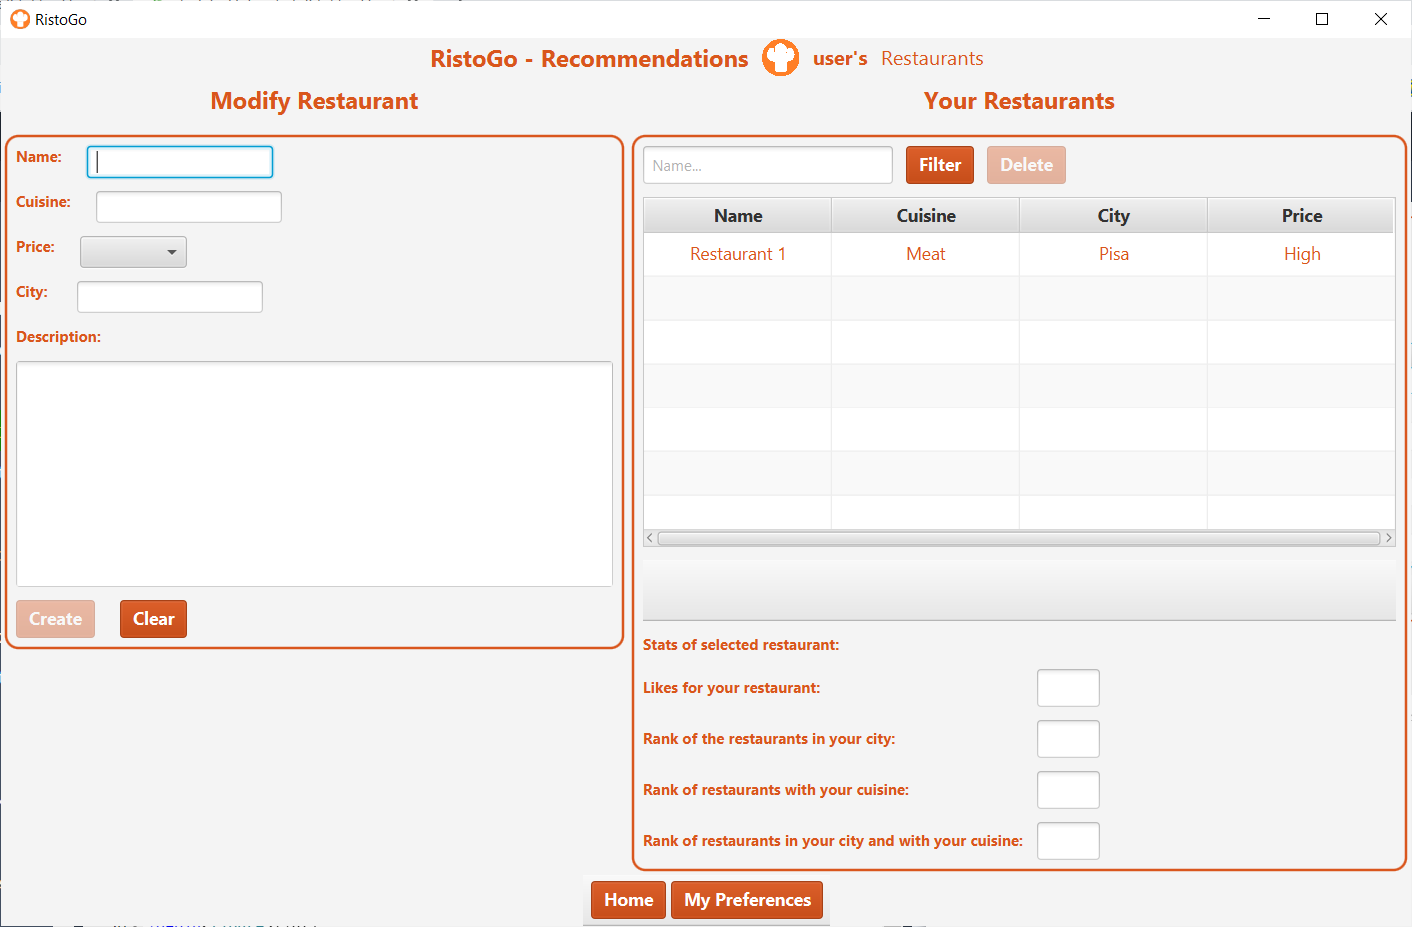
\includegraphics[width=\textwidth]{owner}
	\caption{Owner interface.}\label{fig:owner}
\end{figure}

\subsection{View restaurant's statistics}

Selecting a restaurant, you can see how many likes your restaurant has and its
position considering many rankings: restaurants in the your city, restaurants
with your cuisine and restaurants both in your city and with your cuisine
(\figref{fig:statistics}).

\begin{figure}[H]
	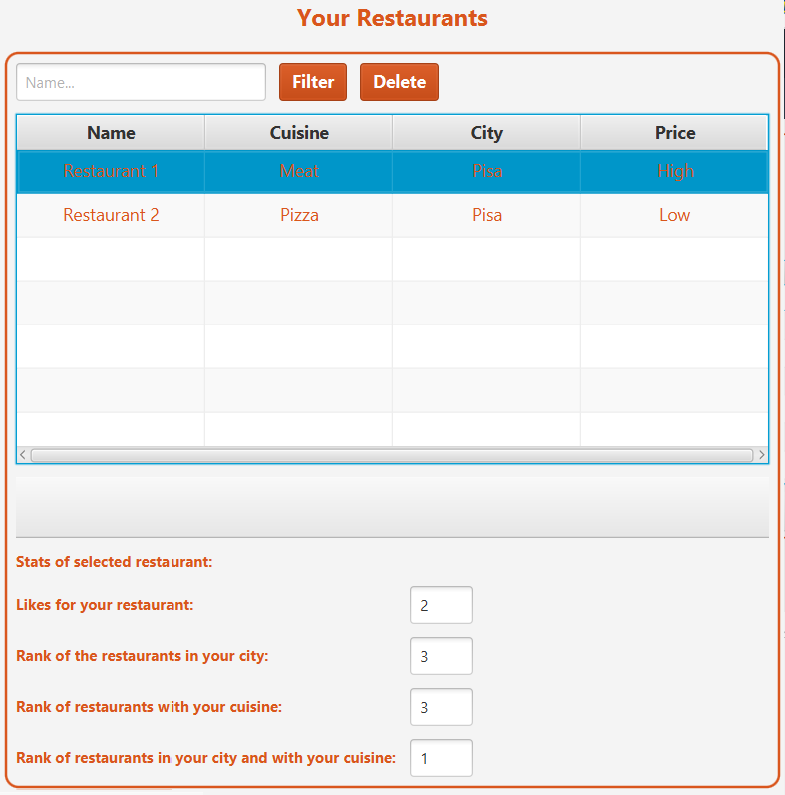
\includegraphics[width=\textwidth]{statistics}
	\caption{Restaurant's statistics.}\label{fig:statistics}
\end{figure}

\subsection{Create a new restaurant}

To create a new restaurant you have to fill the form of the section ``Modify
restaurant'', writing the name, the cuisine, the city and selecting the price
range (\figref{fig:create_restaurant}). Then, click on the button ``create''. If
there are no errors you can see the new restaurant into your restaurants list
(\figref{fig:show_restaurants}).

\begin{figure}[H]
	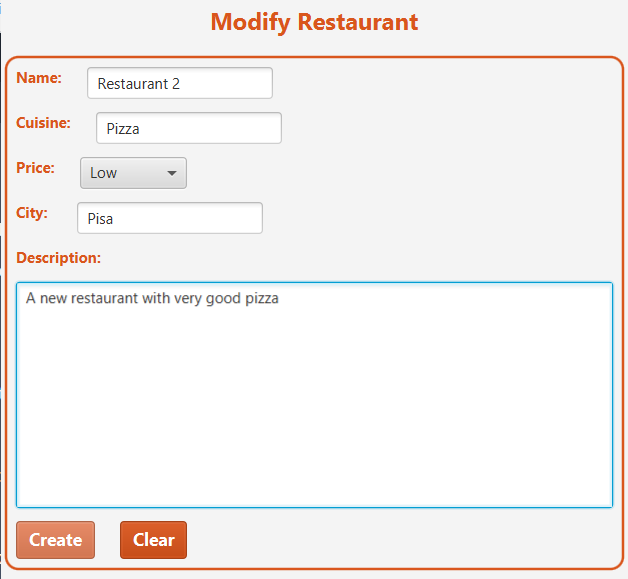
\includegraphics[width=\textwidth]{create_restaurant}
	\caption{Creation of a new restaurant.}\label{fig:create_restaurant}
\end{figure}

\begin{figure}[H]
	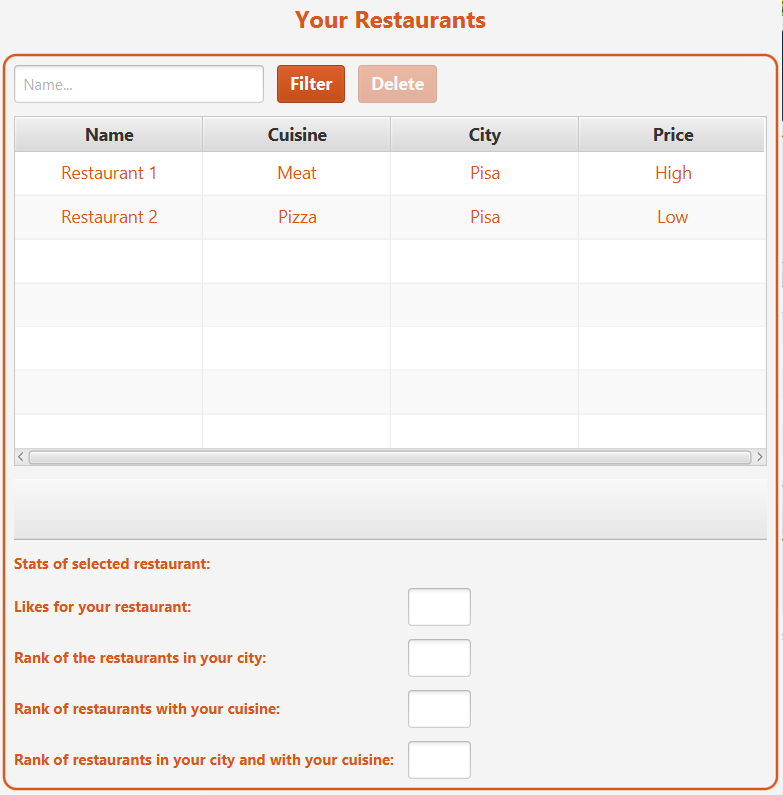
\includegraphics[width=\textwidth]{show_restaurants}
	\caption{List of restaurants after creating a new one.}\label{fig:show_restaurants}
\end{figure}

\subsection{Modify restaurant's information}

After the first creation you can change your restaurant’s information, selecting
it on the Restaurants section and filling the
form on the section ``Modify your restaurant''. Then click on the button
``Commit'' (\figref{fig:modify_restaurants}).

\begin{figure}[H]
	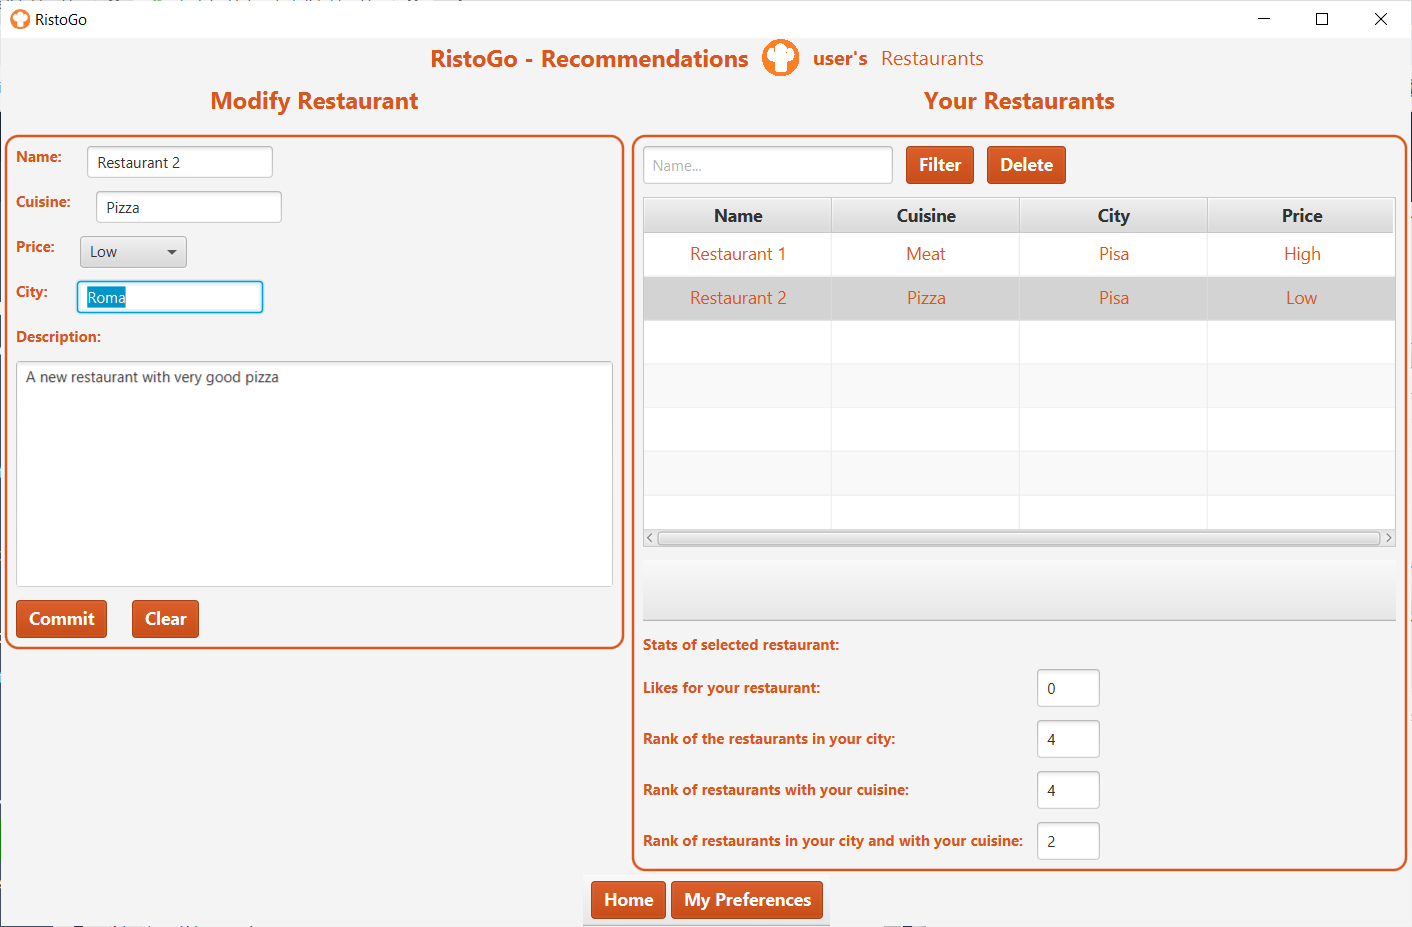
\includegraphics[width=\textwidth]{modify_restaurants}
	\caption{Modify restaurant's information.}\label{fig:modify_restaurants}
\end{figure}

\subsection{Delete a restaurant}

If a restaurant doesn't exist anymore, you can delete it. Click on the right
restaurant and press ``delete'' (\figref{fig:select_restaurant}). If there are
no errors you don't see now the restaurant into your list
(\figref{fig:delete_restaurant})

\begin{figure}[H]
	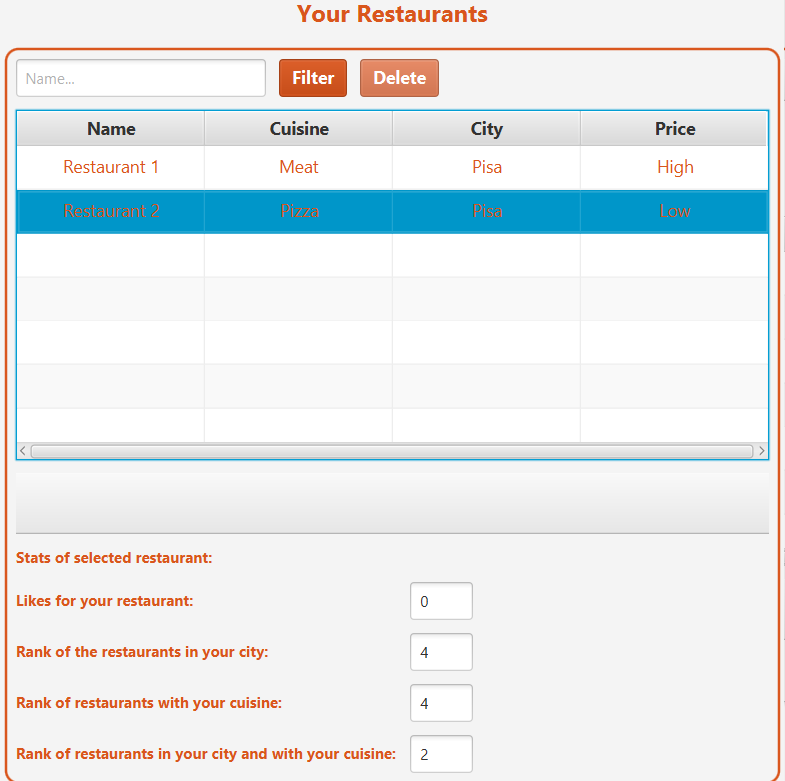
\includegraphics[width=\textwidth]{select_restaurant}
	\caption{Delete a restaurant.}\label{fig:select_restaurant}
\end{figure}

\begin{figure}[H]
	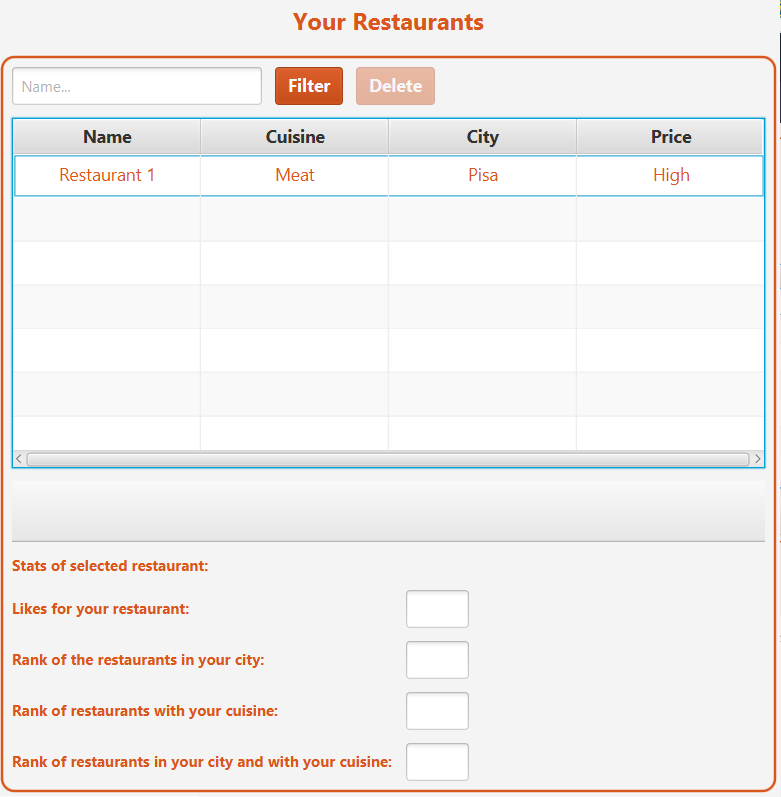
\includegraphics[width=\textwidth]{delete_restaurant}
	\caption{List of restaurants after a delete operation.}\label{fig:delete_restaurant}
\end{figure}
